
\documentclass[conference]{IEEEtran}

\usepackage{rotating}
\usepackage{ifpdf}
\usepackage{algorithmic}
\usepackage{graphicx}
\usepackage{multirow}
\usepackage[TABBOTCAP]{subfigure}
\usepackage{caption}
\usepackage{subfigure}
\usepackage{amsfonts}

\usepackage{latexsym}
\usepackage{amssymb}
\setcounter{tocdepth}{3}
\usepackage{lscape}
\usepackage[usenames]{color}


\ifCLASSINFOpdf


\fi


\hyphenation{op-tical net-works semi-conduc-tor}


\begin{document}

\title{GoBus: Progettazione e Sviluppo di un\rq App a Supporto della Mobilit\`{a}}

\author{\IEEEauthorblockN{Gemma Catolino, Elisa D\rq Eugenio, Davide De Chiara, Alessandra Longo\\Dipartimento di Studi e Ricerche Aziendali -  Management \& Information Technology\\Universit\`{a} degli Studi di Salerno, Fisciano (SA), Italia\\\emph{Tutors:} Pasquale Salza, Andrea De Lucia, Filomena Ferucci}}


\maketitle


\begin{abstract}
Il problema della mobilit\`{a} rappresenta una delle maggiori sfide per i governi di tutto il mondo, a causa dei problemi sempre crescenti che riguardano l\rq inquinamento acustico ed ambientale. Nel corso degli ultimi anni, l\rq Unione Europea ha incentivato, tramite campagne promozionali e stanziamenti di fondi ad hoc, l\rq utilizzo di metodi alternativi per la circolazione delle persone. In questo contesto, i problemi organizzativi legati all\rq utilizzo dei trasporti pubblici nelle citt\`{a}, grandi o piccole che siano, sono particolarmente sentiti. Le informazioni circa orari, corse, linee e fermate non sempre sono facilmente reperibili da parte di chi si trova ad usufruire dei servizi di trasporto. La naturale conseguenza \`{e} rappresentata da disagi di ogni sorta di cui quotidianamente si parla sui mass media. In questo documento viene presentata \emph{GoBus}, un software per la semplificazione delle attivit\`{a} di reperimento delle informazioni da parte dei cittadini. Progettata come un\rq applicazione consultabile sia tramite browser web che come applicazione mobile, \emph{GoBus} consente agli utenti di poter accedere alle informazioni sulla mobilit\`{a} organizzata dai servizi di trasporto di ogni citt\`{a}. L\rq ausilio delle tecniche e dei processi proposti dall\rq Ingegneria del Software ha consentito la realizzazione di un software conforme ai reali bisogni dei cittadini. Inoltre, lo svolgimento del progetto ha seguito le linee guida riguardo la gestione dei progetti software. A supporto di questa idea, \`{e} stata realizzata un\rq applicazione web, con funzione di prototipo, che dimostra la reale fattibilit\`{a} dei requisiti identificati e che illustra un suo possibile utilizzo in un ambiente reale.
\end{abstract}

\IEEEpeerreviewmaketitle



\section{Introduzione}
\label{intro}
Il problema della mobilit\`{a} urbana

\section{Problem Statement}
\label{PS}
La maggior parte delle citt\`{a}, grandi o medie che siano, posseggono una fitta rete di collegamenti. Tali collegamenti il più delle volte appaiono difficili da comprendere e creano spesso confusione sia non solo ai visitatori occasionali, ma anche alle persone più pratiche della citt\`{a}. Nel corso degli anni, il progresso tecnologico ha fatto in modo che fossero sviluppate applicazioni mobile a supporto della fruibilit\`{a} delle informazioni sui collegamenti che le aziende di trasporto forniscono. 
Da allora i più famosi store per smartphone (App Store\footnote{https://itunes.apple.com/us/genre/ios/id36?mt=8}, Google Play \footnote{https://play.google.com/store}, Windows Phone\footnote{http://www.windowsphone.com/it-it/store}) rendono disponibili ogni giorno e con continui aggiornamenti applicazioni mobile, ma queste, per la maggior parte, sono legate solamente alla specifica città e non orientate verso un concetto più ampio come l’intera nazione.\\ 
Avere un’applicazione di carattere nazionale consentirebbe a tutti i cittadini o turisti di essere maggiormente informati su tutta la mobilit\`{a} italiana. Risulterrebbe inoltre pi\`{u} pratica dato che in una sola \emph{app} potrebbero essere consultati e/o programmati orari, linee e percorsi di tutte le corse urbane della propria città o a seconda di dove ci si trova.\\
\emph{Moovit} \footnote{https://itunes.apple.com/it/app/moovit-trasporto-pubblico/id498477945?mt=8} (disponibile per i tre principali store) è una delle poche applicazioni che comprende una vasta scelta di città (all'incirca 20). Rende non solo disponibile informazioni di collegamento riguardo autobus ma anche di treni e metro (qualora presenti). L'applicazione consente di ricercare e di fruire informazioni riguardo ogni tipo di collegamento e pianificare un eventuale viaggio urbano. 
La caratteristica più interessante di questa applicazione è che risulta molto social. Essa infatti reperisce informazioni sulla qualità del percorso della linea di un collegamento (affollamento, orario di arrivo) tramite le valutazione degli utenti. 
Nel suo complesso \emph{Moovit} risulta essere completa e molto utile, in più viene resa appetibile grazie al suo aspetto social, come sopra citato. Tuttavia presenta dei limiti. Navigandola infatti, si mostra inizialmente abbastanza confusionaria in quanto risulta complicato capire come poter usufruire delle funzionalità che essa mette a disposizione. Un altro limite risiede nella sola possibilità di basarsi sulla posizione attuale, escludendo quindi la possibilità di selezionare una diversa città, qualora si voglia prevenire futuri spostamenti in altre metropoli.
Inoltre è ovvio pensare che il servizio \emph{``Social''} (ciliegina sulla torta  dell'applicazione) non potrà essere garantito per sempre, poichè troppo legato all'attività degli utenti.\\
Da questa problematica nasce l’idea di sviluppare \emph{GoBus}, un’applicazione pensata per essere accessibile sia tramite una web application che da dispositivi mobile (ad esempio, Windows Phone).\\
\emph{GoBus} consentirà di avere a disposizione tutti i collegamenti delle citt\`{a} italiane, a seconda di dove ci si trova. Consentirà di dare informazioni sui percorsi da seguire, e in base alla propria posizione visualizzare fermate e linee nelle vicinanze, oppure scegliere comodante da soli una citt\`{a}.
Tutto questo grazie anche alle aziende di trasporti (oltre agli admin dell’applicazione) le quali potranno caricare i dettagli appartenenti ai collegamenti e le varie news associate. Tali file che le aziende caricheranno non saranno lavoro aggiuntivo per loro, dato che si utilizzeranno gli stessi file che le aziende forniscono a Google.
\section{Management}
\label{management}
Dal punto di vista organizzativo del progetto \emph{GoBus}, si \`{e} deciso, grazie alle esperienze acquisite dal team nell\rq ambito del corso di IT Project \& Service Management, di trovare un giusto equilibrio tra il ciclo di vita di un progetto, costituito dalle fasi di ingegnerizzazione e produzione, e il ciclo gestionale costituito invece dalle attivit\`{a} e processi svolti dal team per governare il progetto. Questa fusione di conoscenze ci ha permesso di gestire al meglio il ciclo di vita del progetto. Come linea guida per tali attivit\`{a} \`{e} stato adottato il \emph{Project Management Body of Knowledge} (PMBOK) \cite{PMBOK}, che descrive l\rq insieme delle tecniche e dei processi standard per la gestione di progetti cos\`{i} come definite dal \emph{Project Management Institute}\footnote{http://www.pmi.org}. I processi del Project Management descritti nel \emph{PMBOK} \cite{PMBOK} sono 47 distribuiti in 5 gruppi: nell\rq ambito del progetto \emph{GoBus}, sono stati utilizzati per compiere le seguenti attivit\`{a}:

\begin{itemize}
	\item {\bf{Inizializzazione}}: Raggruppa i processi necessari a selezionare un progetto in relazione a specifici obiettivi di business, definendo obiettivi e modalit\`{a} di gestione del progetto.
	\item {\bf{Pianificazione}}: Finalizzata a circoscrivere l\rq ambito ed i deliverable del progetto, a definire requisiti di ciascun deliverable e a definire un piano di Project Management contenente le informazioni sui vari piani ausiliari per la gestione di tempi, risorse, costi, qualit\`{a}, rischi, e comunicazione.
	\item {\bf{Esecuzione}}: Finalizzata a gestire e sviluppare il progetto, produrre i deliverable concordati.
	\item  {\bf{Monitoraggio e Controllo}}: Serve a valutare l\rq avanzamento dei lavori, a gestire eventuali modifiche e a verificare la qualit\`{a} dei deriverable realizzati.
	\item {\bf{Chiusura}}: Finalizzata a gestire la chiusura del progetto.
\end{itemize}

\subsection{Inizializzazione}
In questa fase \`{e} stato inizializzato il progetto puntando, da un lato, a definire il team e identificare gli stakeholder di progetto, dall\rq altro a definire business need e strategie da attuare. Per quanto riguarda il team, \`{e} stato creato come deliverable il team contract, un documento nel quale sono state definite alcune regole che riguardano la comunicazione e il people management. Per quanto concerne, invece, gli stakeholder, \`{e} stato creato un registro dove memorizzare i vari stakeholder del progetto nel tempo e i loro contatti.\\
Dopo aver creato le basi del team di progetto, si \`{e} definito lo Statement of Work (SoW), che racchiude le caratteristiche che dovr\`{a} avere il progetto, ovvero le \emph{business need}, le funzionalit\`{a} chiave e il piano strategico che si punta ad ottenere con GoBus. Per quanto riguarda i Business needs come definito anche da ITIL® \cite{ITIL}, \emph{``ogni servizio deve avere una giustificazione''} per questo motivo all\rq interno di un progetto \`{e} fondamentale identificarli e renderli protagonisti della strategia di sviluppo del progetto. Tra i Business needs citati nello Statement of work abbiamo ad esempio la fruibilit\`{a} dell\rq informazione, vitale \`{e} la knowledge sharing, ovvero la diffusione della conoscenza e informazione tramite il servizio offerto. Dallo Statement of work \`{e} gi\`{a} possibile iniziare a tirar fuori i requisiti funzionali che saranno successivamente identificati meglio all\rq interno del Requirements Analysis Document.

\subsection{Pianficazione}
Nella fase di Planning si \`{e} racchiuso tutto il lavoro di pianificazione per quanto riguarda le attivit\`{a} di progetto da svolgere. Passo fondamentale \`{e} stato la realizzazione del Software Project Management Plan (SPMP). Per la realizzazione di quest\rq ultimo si \`{e} seguito quello che \`{e} lo standard ISO-IEC-IEEE 16326-2009\footnote{http://standards.ieee.org/findstds/standard/16326-2009.html} cercando di rispettare le voci specificate dallo standard.
Il Software Project Management Plan (SPMP) \`{e} stato realizzato attraverso la collaborazione tra i quattro componenti del team, sulla base delle esperienze maturate dai singoli e da tecniche facilitative quali brainstorming.
In particolare ci si \`{e} basati sul documento di Statement of Work dal quale \`{e} stato possibile comprendere le deliverable del progetto da realizzare incluse nell\rq apposita sezione dell\rq SPMP.
Ovviamente il documento \`{e} stato aggiornato pi\`{u} volte con l\rq avanzare del progetto. In questo senso, lo scope del progetto \`{e} stato ricavato a partire proprio dalle business needs elaborate e descritte nel documento.
A partire da queste si \`{e} quindi potuto elaborare una descrizione dello scope che \`{e} stata inclusa nell\rq SPMP ed in documenti quali il RAD.
Nella sezione Project Context dell\rq SPMP si \`{e} proceduto alla descrizione del modello di processo adottata nell\rq ambito del progetto e alle modalit\`{a} di miglioramento del processo.
Importante \`{e} stata la definizione degli strumenti e delle infrastrutture necessarie al progetto. Tra questi rientrano appunto dei tool collaborativi quali Google Drive, per la comunicazione quali Google Groups, Skype oltre che vari tools di sviluppo software.
Viene inoltre definito il ruolo del Project Manager nell\rq ambito del progetto. Tale ruole viene ricoperto a turno dai diversi membri del team.
In contemporanea, per consentire un adeguato Management dello Scope di progetto, si \`{e} realizzato un Requirements Management Plan (RMP), sottoinsieme dell\rq SPMP. Lo scopo di tale documento \`{e} specificare le modalit\`{a} di raccolta requisiti ed analisi. 
Nel dettaglio, si sono specificati quelli che sono gli strumenti per la specifica dei requisiti, quali ad esempio Word ed Excel, tecniche di Elicitation quale la preparazione di interviste e tecniche di Analisi dei requisiti quali brainstorming, prototipazione, prioritizzazione etc.
Nel nostro caso per la raccolta dei requisiti si \`{e} scelto di effettuare delle interviste piuttosto che utilizzare una tecnica etnografica che avrebbe portato via tempo e non avrebbe condotto a risultati immediati, soprattutto in vista del fatto che l\rq app finale \`{e} orientata ad una vasta gamma di utenti. Non \`{e} stato possibile effettuare nemmeno alcun benchmarking rispetto ad altri progetti simili, per via delle nostre esigue esperienze.
Per la prioritizzazione dei requisiti si \`{e} deciso di utilizzare tre categorie di valutazione qualitative: alto, medio, basso. In modo da individuare immediatamente su quali requisiti e funzionalit\`{a} concentrare gli sforzi. 
Se pur lo scope di progetto \`{e} risultato chiaro sin dalle primissime fasi, fondamentale \`{e} stata la definizione di un Change Management per quanto concerne i requisiti. In particolare nella definizione delle figure preposte all\rq accettazione dei cambiamenti e alla valutazione dell\rq impatto che tali cambiamenti hanno sul sistema.
In ultimo si \`{e} definita e specificata una Requirements Traceability Matrix (RTM) che ci consente di tener traccia dei requisiti per tutta la durata del progetto e quindi poter verificare l\rq impatto di un cambiamento sul sistema. 
All\rq interno della stessa si va a definire il codice del requisito, un rationale che motiva il requisito, la fonte, l\rq autore, la data di raccolta, una priorit\`{a} ed uno status, oltre a vari riferimenti del requisito all\rq interno dei diversi documenti e del codice sorgente.
Il seguente \`{e} un esempio di macro requisito specificato nell\rq RTM:
\\
\begin{figure}[h]
\centering
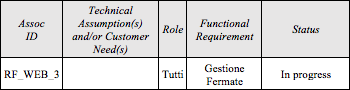
\includegraphics[scale=.7]{img/1.png}
\label{fig:cd}
\end{figure}
\\
\begin{figure}[h]
\centering
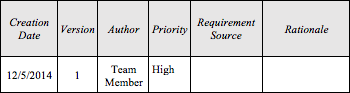
\includegraphics[scale=.7]{img/2.png}
\label{fig:cd}
\end{figure}
\\
\begin{figure}[h]
\centering
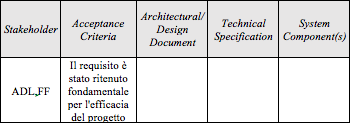
\includegraphics[scale=.7]{img/3.png}

\label{fig:cd}
\end{figure}
\\
\begin{figure}[h]
\centering
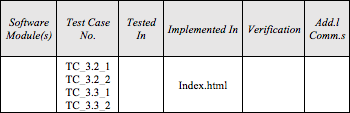
\includegraphics[scale=.7]{img/4.png}
\caption{Esempio di RTM}
\label{fig:cd}
\end{figure}
\\
Nella tabella ADL e FF rappresentano rispettivamente il prof. Andrea De Lucia e la proff.ssa Filomena Ferrucci ritenuti nell\rq ambito del progetto stakeholder e top management.
Il Requirements Management Plan \`{e} risultato quindi fondamentale per la definizione del RAD, descritto nella sezione Software, in cui vengono appunto specificati tutti i requisiti.
Con la realizzazione dell\rq RMP e parallelamente all\rq attivit\`{a} di raccolta requisiti si \`{e} proceduto alla redazione del Software Configuration Management Plan (SCMP). Questa scelta risiede nel fatto che il RAD risulta essere il documento fondante del progetto e che appunto forma la base da cui partire. Modifiche a requisiti dovrebbero essere approvati mediante accettazione formale, soprattutto se queste possono impattare gravemente sul sistema.
Per cui prima di procedere alla realizzazione del RAD \`{e} buona norma predisporre un SCMP. 
Viste le ridotte dimensioni del team lo stesso \`{e} incaricato di valutare i cambiamenti da apportare a Configuration Items baselined.
Nello specifico, il Project Manager di turno \`{e} il Configuration Manager designato. Il ruolo di sviluppatore e auditor \`{e} di volta in volta assegnato a membri del team diversi.
Change Control Board \`{e} l\rq intero team che \`{e} incaricato di valutare l\rq impatto e schedulare le modifiche da apportare.
I Configuration Items (CI) vengono quindi decisi nelle primissime fasi del progetto. Tra questi \`{e} risultato necessario includere: 
\begin{figure}[h]
\centering
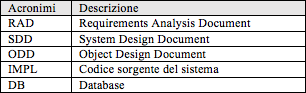
\includegraphics[scale=.7]{img/5.png}
\caption{Configuration Item}
\label{fig:cd}
\end{figure}
Ovviamente altri CI possono essere inclusi in ogni momento se ritenuto necessario.
Le richieste formali di cambiamento non sono schedulate, e possono quindi essere fatte in qualsiasi momento. Questa scelta \`{e} motivata dal fatto che lo scope del progetto \`{e} ben chiaro cos\`{i} come i requisiti iniziali, per cui modifiche in corso d\rq opera non vanno a stravolgere il sistema progettato.
Fondamentale \`{e} risultata anche la scelta di un repository software sul quale \`{e} possibile tener traccia delle diverse versioni del software, tra cui appunto le versioni baselined. Lo stesso DB verr\`{a} caricato su repository insieme al codice sorgente e le versioni baselined verranno specificate in appositi documenti, cos\`{i} come le richieste formali di cambiamento e delle modifiche apportate alle baseline.
Ovviamente per modifiche ai requisiti si pu\`{o} far riferimento alla sezione di Change Management specificata nell\rq RMP.
Per la redazione del documento si \`{e} fatto riferimento allo Std. 828-1990 in versione down-tailored viste le dimensioni del progetto.
Il Configuration Management Plan consente quindi di mantenere il progetto all\rq interno dello scope e questo \`{e} il motivo per il quale si \`{e} deciso di svilupparlo in contemporanea con la fase di raccolta requisiti consentendo l\rq implementazione del Configuration Management come funzione di progetto.
Con la raccolta requisiti e l\rq analisi di quest\rq ultimi si \`{e} quindi definito la versione relativa del RAD come baselined.
A partire da questa, insieme con lo scope definito in precedenza, si \`{e} proceduto alla realizzazione di una baseline dello scope di progetto in base al quale valutare gli avanzamenti, dapprima con la realizzazione di una Work Breakdown Structure (WBS) ed in seguito con la realizzazione di uno scheduling delle attivit\`{a}.
Per quanto riguarda la WBS, essa \`{e} stata realizzata mediante brainstorming da parte del team prendendo in considerazione lo scope, i requisiti, le conoscenze del team e procedendo per analogia rispetto ad altre WBS costruite in precedenza.
In particolare \`{e} stato utile un misto di approcci di visualizzazione tra funzionale e per componenti di progetto. Nel primo caso ci si \`{e} serviti dei 5 process groups definiti dal PMI nel PMBOK 5, nel secondo caso ci si \`{e} basati sia su documenti di Management che tipici dell\rq Ingegneria del Software.
Questo approccio ci ha consentito di rilevare alcuni dettagli non rilevati in prima battuta. 
Il formato finale della WBS \`{e} di tipo gerarchico. Ovviamente si tratta di una WBS grossolana che verr\`{a} raffinata con l\rq avanzare del progetto. Non risulta infatti critica la definizione con largo anticipo dei task e delle responsabilit\`{a} sui singoli task se non per stima dei tempi di progetto.
La figura \ref{fig:wbs} mostra la WBS elaborata.

\begin{figure*}[tp]
\centering
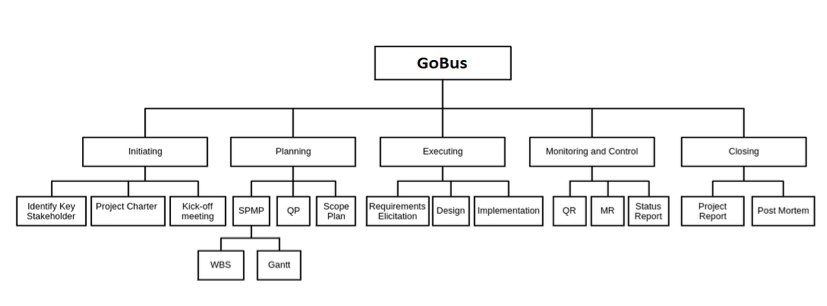
\includegraphics[scale=.6]{img/6.png}
\caption{WBS}
\label{fig:wbs}
\end{figure*}

Sulla base di quest\rq ultima si \`{e} poi passato alla realizzazione dello scheduling delle attivit\`{a}.
Come gi\`{a} accennato in precedenza alcune attivit\`{a} sono state effettuate in contemporanea con altre. Dall\rq esperienza maturata su progetti precedenti si \`{e} riuscito stabilire una durata approssimativa delle diverse attivit\`{a}, soprattutto relative alla fase di initiating e planning.
Inoltre \`{e} stato considerato uno slack time aggiuntivo per le diverse attivit\`{a}.
Per la schedulazione (presente nell\rq SPMP in allegato) si \`{e} tenuto principalmente conto delle deadline imposte da Score-IT e dagli impegni relativi allo studio di ogni componente del team.
Si \`{e} inoltre tenuto conto anche della presenza, fondamentale, di un corso di sviluppo applicazioni mobili al secondo semestre, per cui la fine del progetto \`{e} stata prevista per il 30/06/2015.
Sia la WBS che lo scheduling vengono specificate nella sezione Project Planning dell\rq SPMP. In questa sezione viene inoltre specificato, tra i vari aspetti, quello legato al training.
Infatti la realizzazione di un\rq applicazione per \emph{Windows Phone} comporta l\rq apprendimento da parte dei membri del team di tecnologie non conosciute al momento, tra cui \emph{C\#} e la conoscenza dell\rq ambiente di sviluppo \emph{.NET}. In contemporanea con la realizzazione della WBS si \`{e} proceduto con la realizzazione del Quality Plan (QP). Il Quality Plan (QP) \`{e} stato redatto in questa fase del progetto in quanto \`{e} importante avere uno scope chiaro e dei requisiti funzionali e non funzionali chiari in modo da rispettare degli obiettivi di qualit\`{a} che si relazionino ai requisiti. Per cui la base di tale QP \`{e} stato il RAD, l\rq SPMP e lo SoW.
Lo standard di riferimento \`{e} stato ISO/IEC 9126 che definisce un modello di qualit\`{a} del software. In particolare, tale standard definisce sei categorie di qualit\`{a}, ulteriormente suddivise in sotto categorie secondo una struttura gerarchica. Si \`{e} deciso di dare una forte rilevanza all\rq aspetto della funzionalit\`{a} soprattutto per quanto riguarda l\rq accuratezza.
Questo consentir\`{a} agli utenti finali di poter ottenere le informazioni nel modo pi\`{u} dettagliato e preciso possibile, tenendo ovviamente conto di aspetti collegati alla sicurezza delle informazioni sensibili dell\rq utente ed una adeguatezza delle funzionalit\`{a} a quello che \`{e} lo scopo del sistema.
Si \`{e} deciso inoltre di garantire un\rq alta operabilit\`{a} garantendo all\rq utente un alto controllo delle funzionalit\`{a} oltre che fornire un buon grado di apprendibilit\`{a}.
Da come si potr\`{a} evincere dai mock-up allegati al RAD l\rq applicazione risulter\`{a} particolarmente semplice ed immediata.
Particolare importanza \`{e} stata data all\rq aspetto di comportamento temporale. Il sistema infatti dovr\`{a} essere in grado di fornire una risposta in tempi particolarmente brevi, 1-2 sec.
Questo ovviamente comporter\`{a} l\rq utilizzo di tecnologie particolarmente performanti, non utilizzate per la prima prototipazione ma utilizzate in seguito e specificate nella sezione Software.
Inoltre l\rq aspetto collegato alla manutenzione \`{e} stato ritenuto fondamentale. Il garantire infatti il servizio agli utenti nel corso del tempo dipende da un elevato grado di manutenibilit\`{a} del sistema e quindi di una modularit\`{a} e grado di design elevato del sistema stesso.
Importante \`{e} stata la definizione di quelli che sono i ruoli per garantire un corretto Quality Management mostrati in \emph{figura 4}.
\begin{figure*}[tp]
\centering
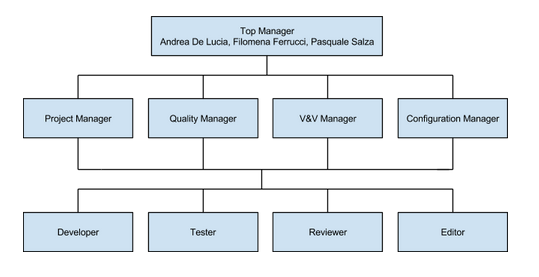
\includegraphics[scale=.6]{img/10.png}
\caption{Organizzazione team}
\label{fig:cd}
\end{figure*}
Si \`{e} deciso di stabilire il ruolo di un Verification \& Validation Manager in modo da garantire la redazione di checklist \emph{ad hoc} per artefatto sulla base di quanto specificato nel QP.
Oltre alla definizione dei ruoli, nel QP \`{e} stato anche definito un Communication Plan. Questo definisce le modalit\`{a} di comunicazione tra i membri di tipo formale, ovvero tramite Google Groups.
Nel QP viene inoltre definito il workflow che la redazione dei documenti segue nel progetto. Il seguente grafico mostra lo schema adottato:
\begin{figure}[tp]
\centering
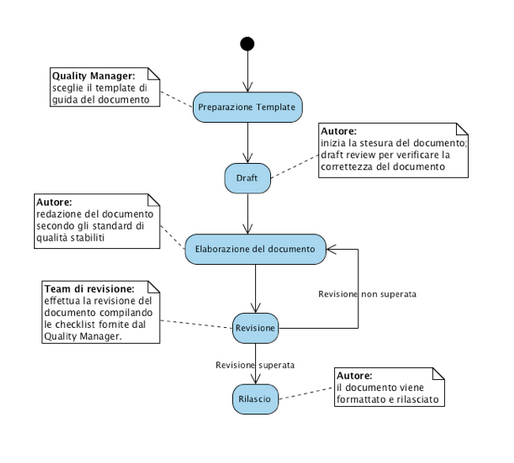
\includegraphics[scale=.5]{img/11.png}
\caption{Workflow qualit\`{a}}
\label{fig:cd}
\end{figure}
Compito del Quality Manager \`{e} quindi quello di definire dei Template da utilizzare per i documenti. Tali template sono quindi utilizzati dai membri del team nella redazione dei documenti.
In questo caso il documento viene definito come draft. Terminata l\rq elaborazione \`{e} compito del team di revisione predisposto effettuare una revisione formale del documento sulla base delle checklist preparate dal Quality Manager o dal V\& V Manager. 
Se tale revisione ha esito positivo il documento pu\`{o} essere rilasciato, altrimenti deve essere modificato rispettando quella che \`{e} la checklist compilata dal team di revisione predisposto.
Nel nostro caso il ruolo di team di revisione spetta ad uno o due membri designati dal project manager incaricati di rivedere un documento. Ovviamente nel team non rientra il membro redattore del documento in questione.
Si \`{e} deciso di specificare, in ogni documento, una revision history indicando redattore, data e tipologie di modifiche effettuate, una pagina di intestazione indicante titolo del documento, nome progetto, versione. 
Inoltre vengono indicati font da utilizzare, grandezza, tipologie di intestazioni di paragrafi etc.
Per quanto concerne il software al momento non sono state specificate modalit\`{a} di verifica dello stesso. Questo \`{e} dovuto alla non conoscenza delle tecnologie che saranno adoperate, in particolare \emph{C\#} e l\rq ambiente \emph{.NET}, per cui al momento non risulta facile prendere delle decisioni in merito.
Tuttavia, considerato che \emph{C\#} presenta notevoli similitudini con il linguaggio \emph{Java} si pu\`{o} pensare di utilizzare delle metriche statiche del codice oltre che delle metriche specifiche per linguaggi ad oggetti.
Sicuramente come parametro verr\`{a} tenuto in considerazione la presenza di commenti a metodi, classi e variabili ove queste non siano di immediata comprensione.
Per il reporting e l\rq issue tracking del codice si utilizzeranno i sistemi integrati in BitBucket, la piattaforma web utilizzata per la gestione del repository del codice sorgente nell\rq ambito del progetto.
Dal momento che tale documento \`{e} stato redatto insieme col Risk Management Plan (RiMP) \`{e} risultato altrettanto rilevante includere in una apposita sezione del QP i rischi riguardanti la qualit\`{a} di progetto:
\begin{figure}[h]
\centering
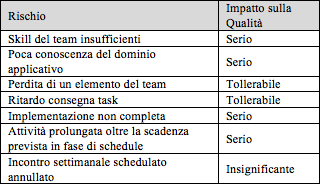
\includegraphics[scale=.7]{img/12.png}
\caption{Rischi}
\label{fig:cd}
\end{figure}
L\rq impatto sulla qualit\`{a} \`{e} riportato in categorie qualitative da Serio a Insignificante, dal pi\`{u} grave al meno grave.
Come gi\`{a} detto in precedenza, visto il legame tra Quality e Verification and Validation, i due plan sono stati redatti parallelamente.
Il V\& V Plan ha lo scopo di predisporre delle linee guida per la verifica e la validazione di un artefatto prima di essere definito baselined.
La fase di verifica e validazione degli artefatti prodotti durante lo sviluppo del sistema, prevede l\rq utilizzo di checklist di revisione. Per ogni artefatto sottoposto a revisione verr\`{a} definita una checklist specifica. 
Per cui vi sar\`{a} una fase di pianificazione in cui verranno elaborate le checklist e selezionati dei membri per la revisione, seguita da una fase di definition in cui vi sar\`{a} la realizzazione fisica del template della checklist, messo a disposizione di tutti.
Nella fase di review i revisori hanno il compito di verificare che l\rq artefatto sia conforme a quanto definito nel QP.
Se l\rq artefatto non \`{e} accettato allora vi \`{e} una fase di rework in cui esso deve essere adeguato rispetto a quanto stabilito nella checklist.
Il diagramma seguente riporta le fasi del processo di revisione degli artefatti prodotti nell\rq ambito del progetto del sistema:
\begin{figure}[h]
\centering
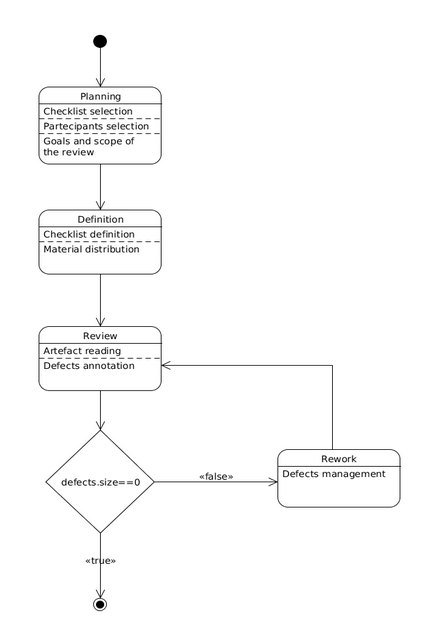
\includegraphics[scale=.6]{img/13.png}
\caption{Diagramma fasi di revisione}
\label{fig:cd}
\end{figure}
Alcune checklist vengono proposte in seguito nel documento. Ovviamente tali checklist e quindi monitoraggio degli artefatti, rientra nella normale esecuzione delle fasi del progetto cos\`{i} come descritto nel PMBOK 5 e nello specifico nella fase di Monitoring and Controlling.
Il QP e il VVP fanno s\`{i} che venga aggiornata la sezione 8 del SPMP nella quale rientrano informazioni sulla verifica e validazione e qualit\`{a}.
La rilevanza data all\rq aspetto della qualit\`{a} rientra nell\rq ottica dell\rq ottenimento di un prodotto che sia conforme a quelle che possano essere le aspettative dell\rq utente finale.
Inoltre consentir\`{a} una coerenza e consistenza per quanto riguarda lo scope di progetto, per cui deviazioni saranno evitate.
Aspetto negativo pu\`{o} essere l\rq introduzione di una eccessiva burocrazia in quello che dovrebbe essere uno sviluppo basato su tecniche agili. Tuttavia si far\`{a} in modo che tali processi di verifica non blocchino eccessivamente il processo di sviluppo del sistema.
Un ulteriore sforzo da parte del team \`{e} stato fatto per la creazione del Risk Management Plan (RiMP).
Seppur il progetto \`{e} di piccole dimensioni si \`{e} ritenuto fondamentale predisporre un piano per l\rq identificazione, la valutazione, il monitoraggio dei rischi.
Infatti nonostante la nostra breve esperienza dai precedenti corsi \`{e} subito risultato evidente come il sottovalutare dei rischi ha portato in seguito a problemi, come ritardi nei tempi di consegna o addirittura fine prematura del progetto.
Innanzitutto si \`{e} proceduto con l\rq individuare delle categorie di valutazione per quanto riguarda la probabilit\`{a} e l\rq impatto di un rischio.
Un primo meeting ci ha quindi portato a categorizzare la probabilit\`{a} di accadimento di un rischio e il suo impatto.
Attraverso una fase di brainstorming e benchmarking con progetti precedenti si sono identificati una serie di rischi da valutare. 
In un ulteriore meeting, un moderatore ha sottoposto ad ogni membro del team la lista dei rischi chiedendo di valutarne l\rq impatto e la probabilit\`{a}. Le risposte anonime, sono state raccolte effettuandone una convergenza verso valori unici.
Per alcuni rischi \`{e} stato necessaria altra discussione, per altri invece la convergenza era ampia. Questa tecnica viene definita come tecnica Delphi.
La risultante \`{e} la seguente tabella dei rischi:
\begin{figure}[h]
\centering
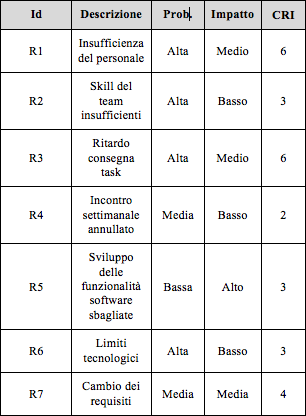
\includegraphics[scale=.6]{img/17.png}
\caption{Tabella dei rischi}
\label{fig:cd}
\end{figure}
Il rischio riguardante gli skills insufficienti \`{e} stato ritenuto di impatto basso in quanto i membri del team hanno effettuato un\rq autovalutazione asserendo di essere in grado di colmare il gap in tempi brevi. Questo supportato soprattutto dalla presenza di un corso di Sviluppo Applicazioni Mobili al secondo semestre.
Per ogni rischio \`{e} stato predisposto un breve piano di contingenza da attuare nel caso si verifichi e delle azioni per mitigare i trigger che scatenano i rischi. Vista la dimensione del progetto e l\rq assenza di un budget economico non si \`{e} ritenuto necessario predisporre piani dettagliati.
\begin{figure}[h]
\centering
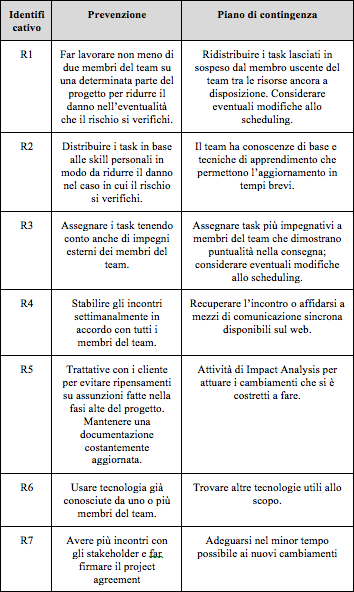
\includegraphics[scale=.6]{img/18.png}
\caption{Piano di contigenza}
\label{fig:cd}
\end{figure}
Il RiMP oltre a comportare un aggiornamento dell\rq SPMP, ha permesso la creazione di un Risk Register (RiR) sul quale sono riportati i rischi da monitorare durante la fase di esecuzione del progetto.
Il RiR verr\`{a} aggiornato costantemente mano a mano che il progetto progredisce, aggiornando sia la probabilit\`{a} di accadimento sia l\rq impatto.
Da quanto descritto finora si pu\`{o} notare come l\rq SPMP subisca modifiche mano a mano che i vari piani vengono elaborati. Altra sezione da considerare \`{e} la definizione della consegna del prodotto. Cos\`{i} come specificato sin dalla prima definizione dell\rq SPMP, il prodotto \`{e} dapprima prototipato con una versione web-based in cui sono presenti alcune funzionalit\`{a} di base, successivamente tale prototipo verr\`{a} evoluto creando la versione finale del sito web, accompagnata da un app principale per Windows Phone. Entrambe si interfacceranno con un web service restful.

\subsection{Esecuzione}
Durante la fase di esecuzione, cos\`{i} come definito nello scheduling, vengono elaborate le deliverable principali:\\
\begin{itemize}
\item SDD
\item ODD
\item Codice Sorgente:
\begin{itemize}
\item Web Service
\item App per Windows Phone
\item Web application
\end{itemize}
\item Database
\item Test Plan
\end{itemize}
La base di partenza \`{e} ovviamente tutta la documentazione di Management prodotta nella fase di Initiating e Planning. Fondamentale risulta il RAD da cui partire per una prima decomposizione del sistema in sottosistemi.
Questa fase verr\`{a} quindi descritta in dettaglio nella sezione riguardante il software in cui sono descritti i vari documenti riportati sopra tra cui il RAD.


\subsection{Monitoraggio e Controllo}
Il monitoraggio e controllo \`{e} una fase che ha inizio insieme alla fase di pianificazione e dura fino alla fase di chiusura, \`{e} una fase dove si valuta l\rq avanzamento dei lavori e si attua il piano che \`{e} stato concepito nel Verification \& Validation Plan seguendo le metriche di misurazione di qualit\`{a} definite nel Quality Plan. In pratica durante le fasi di pianificazione e esecuzione tramite l\rq utilizzo di checklist definite nel V \& V si revisionano i documenti creati. Vi sono diverse tipologie di checklist quelle per i documenti, dove vi \`{e} un componente del team che compila le checklist e quando termina invia le checklist al creatore del documento che la controlla e decide di accettarla e apportare le modifiche richieste. Di seguito il template utilizzato per la checklist di revisione dei documenti:\\

\begin{figure}[h]
\centering
\includegraphics[scale=.45]{img/checklist.png}
\caption{Checklist valutazione generica documento}
\end{figure}

Altre tipologie di checklist che abbiamo definito sono per la raccolta e analisi dei requisiti, stima dei costi e dei tempi, software configuration management, risk management, quality assurance e  testing. La compilazione di queste checklist da parte del team porta a una chiara misurazione della qualit\`{a} del progetto, per maggiori dettagli sulle checklist invito a consultare il documento Verification \& Validation Plan. Dopo questa analisi che ci ha permesso di monitorare il progetto sono stati redatti dei management e quality report per capire appunto cosa doveva essere revisionato e aggiornato, un esempio nel quality report:\\
 
\begin{figure}[!h]
\centering
\includegraphics[scale=.45]{img/risultato.png}
\caption{Risultato Checklist specifica}
\end{figure}

Dove B sta a indicare che il documento \`{e} stato accettato ma vanno apportate lievi modifiche.

\subsection{Chiusura}
Una volta che arriveremo alla fase di chiusura di progetto e quindi aver ottenuto il risultato sulla base delle specifiche date in input, si proceder\`{a} con la stesura della post-mortem review ovvero un deliverable per analizzare gli elementi del progetto e capire se sono stati di successo o di insuccesso. Dopo aver dato il proprio giudizio vi sono una serie di domande aperte che riguardano lesson learned e considerazioni finali.
La post-mortem review ci aiuter\`{a} nel gestire futuri rischi gi\`{a} incotrati in questo progetto quindi migliorando le nostre skill dal punto di vista del risk management e delle Best Practice.



\section{Software}
\label{software}
Questa sezione descrive il processo di sviluppo adottato nell\rq ambito del profetto \emph{GoBus}.

\subsection{Modello del Ciclo di Vita}
In base alle esigenze relative alle tempistiche e agli obiettivi del progetto, il modello del ciclo di vita che meglio si adatta \`{e} il ciclo \emph{evolutivo a prototipazione}. In particolare, vista la necessita di comprendere meglio i requisiti che il committente richiedeva, la tecnica utilizzata consente di fornirgli un prototipo del sistema in tempi rapidi. In questo modo, \`{e} possibile periodicamente avere feedback utili per la continuazione delle attivit\`{a} progettuali.

\subsection{Requirement Elicitation and Analysis}
La fase di requirement elicitation consiste nella comprensione delle necessit\`{a} del committente, al fine di collezionare i requisiti del sistema. Nell\rq ambito del progetto, tale attivit\`{a} \`{e} stata svolta facendo brainstorming con tutti gli stakeholder interessati. In particolare, sono stati organizzati incontri sia con i coordinatori del progetto sia con aziende di trasporto locali. Per mitigare il richio di errata comprensione delle reali necessit\`{a} degli stakeholder, i meeting si sono ripetuti cos\`{i} che, ad ogni incontro, i requisiti potessero essere meglio fissati. Il numero totale di incontri con gli stakeholder \`{e} 3.\\
La tabella \ref{tab:gestioni} mostra, ad alto livello, i principali raggruppamenti delle funzionalit\`{a} identificate nell'ambito del progetto \emph{GoBus}. Di seguito verr\`{a} analizzato in dettaglio ciascun raggruppamento. Si noti che per evitare ridondanza e per ragioni di spazio, non sono riportati tutti i requisiti funzionali identificati. Per la lista completa, si faccia riferimento al Documento di Analisi dei Requisiti (RAD) in allegato.\\

\begin{table*}[tb]
   \centering
   \caption{Overview delle Funzionalit\`{a} Identificate}
   \label{tab:gestioni}
  \resizebox{1\linewidth}{!}{
   \begin{tabular}{ll}\hline
   Nome & Descrizione\\\hline
   Gestione Registrazione & Insieme di funzionalit\`{a} che consentono la registrazione di un nuovo utente.\\
   Gestione Autenticazione & Insieme di funzionalit\`{a} che consente il riconoscimento degli utenti registrati.\\
   Gestione Account & Insieme di funzionalit\`{a} per la manipolazione degli account degli utenti.\\
   Gestione Fermate & Funzionalit\`{a} che consente di visualizzare le fermate tramite l\rq applicazione di diversi filtri per la ricerca mirata.\\
   Gestione Linee & Funzionalit\`{a} che consente la visualizzazione delle linee tramite l\rq applicazione di diversi filtri per la ricerca mirata.\\
   Gestione Percorso & Insieme di funzionalit\`{a} che consente la visualizzazione delle indicazioni stradali.\\
   Gestione Preferiti & Funzionalit\`{a} che consente la gestione delle fermate e delle linee preferite.\\
   Gestione News & Insieme di funzionalit\`{a} per la efficace gestione degli avvisi da parte delle aziende di trasporti.\\
   Gestione Dati GTFS & Insieme di funzionalit\`{a} che consente ad un\rq azienda di trasporti di caricare il proprio file GTFS.\\
   \hline
   \end{tabular}
   }
\end{table*}

\noindent {\bf{Gestione Registrazione}}: La gestione della registrazione da la possibilit\`{a} ad un nuovo utente di potersi iscrivere alla piattaforma. Vale la pena notare che la registrazione \`{e} consentita i) utilizzando la propria e-mail, fornendo un nickname ed una password; ii) tramite l'utilizzo dell'account Facebook; iii) tramite l'utilizzo dell'account Google. Questo insieme di requisiti \`{e} comune sia alla parte relativa alla web application che all'applicazione mobile.
\noindent {\bf{Gestione Autenticazione}}: Questa gestione permette ad un utente registrato di essere riconosciuto e abilitato a effettuare determinate operazioni da parte del sistema. Quindi, le funzionalit\`{a} di login e logout fanno parte di questa gestione.\\

\noindent {\bf{Gestione Account}}: Questo insieme di funzionalit\`{a} si occupa di tutto ci\`{o} che ha a che fare con la manipolazione delle informazioni personali degli utenti registrati al sistema. Nel dettaglio, \`{e} possibile visualizzare, modificare ed eliminare un account dalla piattaforma.\\

\noindent {\bf{Gestione Fermate}}: Questa funzionalit\`{a} permette di visualizzare le fermate tramite l\rq applicazione di diversi filtri, al fine di effettuare una ricerca mirata delle informazioni di cui l\rq utente necessita. I requisiti funzionali identificati riguardano la visualizzazione delle fermate tramite i) geo-localizzazione della posizione dell'utente; ii) una localit\`{a} specifica; o iii) nome della localit\`{a}. Inoltre, \`{e} possibile visualizzare le linee relative ad una fermata, consentendo quindi di conoscere, data una fermata, quali linee la percorrono.\\

\noindent {\bf{Gestione Linee}}: Questa funzionalit\`{a} permette di visualizzare le linee tramite l\rq applicazione di diversi filtri per effettuare una ricerca mirata delle informazioni di cui l\rq utente necessita. Sar\`{a} consentita la visualizzazione delle: linee di una specifica localit\`{a}, ma anche la ricerca di una linea e la visualizzazione di tutte le corse di una linea con i relativi orari di andata e ritorno. Inoltre, sar\`{a} implementata anche la visualizzazione dell'intero percorso di una determinata corsa.\\

\noindent {\bf{Gestione Percorso}}: Questa funzionalit\`{a} da all'utente la possibilit\`{a} di richiedere la navigazione tra un punto di partenza ed uno di arrivo.\\

\noindent {\bf{Gestione Preferiti}}: Tramite questa funzionalit\`{a} l'utente avr\`{a} la possibilit\`{a} di memorizzare le sue corse, linee, e citt\`{a} preferite, cos\`{i} da poter rapidamente accedere a tali informazioni in futuro.\\

\noindent {\bf{Gestione News}}: Questa funzionalit\`{a} \`{e} implementata esclusivamente per la parte riguardante la web application e consente ad una azienda di trasporti di poter inserire, modificare ed eliminare avvisi.\\

\noindent {\bf{Gestione dati GTFS}}: Questa funzionalit\`{a} \`{e} implementata esclusivamente per la parte riguardante la web application e consente ad una azienda di trasporti di poter caricare il proprio file GTFS.

L'analisi dei requisiti \`{e} poi proceduta tramite la modellazione delle funzionalit\`{a} identificate in casi d\rq uso. In questo documento, verr\`{a}  proposto un solo caso d\rq uso, cos\`{i} da consentire al lettore di poter comprendere la metodologia di modellazione adottata. In particolare, verr\`{a}  seguita la modellazione del requisito riguardante la ricerca di una linea. 

\begin{figure*}[tb]
\centering
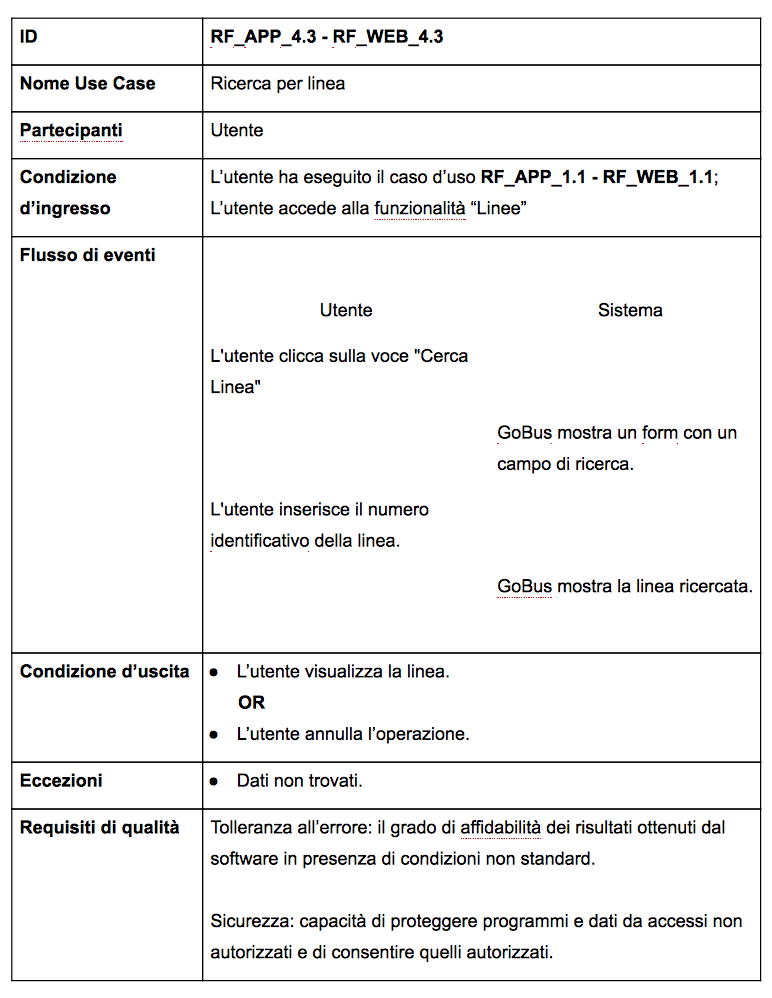
\includegraphics[scale=.7]{img/cd.png}
\caption{Caso d\rq uso relativo al requisito funzionale che consente la ricerca di una linea.}
\label{fig:cd}
\end{figure*}

La Figura \ref{fig:cd} mostra il caso d\rq uso relativo al requisito funzionale che consente la ricerca di una linea. In particolare, l'utente registrato, dopo aver effettuato l'accesso al sistema (condizione d\rq entrata necessaria), clicca sul tasto che consente la ricerca di una linea e digita la query di ricerca prescelta. Il sistema acceder\`{a} all'archivio dati e caricher\`{a} la linea ricercata. Vale la pena notare che ogni caso d\rq uso del sistema modella un requisito sia considerando le azioni che intercorrono tra l\rq utente e il sistema, sia considerando i requisiti di qualit\`{a} ed eventuali condizioni che potrebbero causare eccezioni.\\

Il successivo step nella modellazione delle funzionalit\`{a} del sistema \`{e} consistito nella definizione dei path navigazionali relativi a ciascun raggruppamento di requisiti identificato. Di seguito \`{e} mostrato il path navigazionale che consente ad un utente registrato di muoversi all\rq interno della gestione delle linee, di cui il requisito di ricerca delle linee \`{e} incluso.

\begin{figure}[!h]
\centering
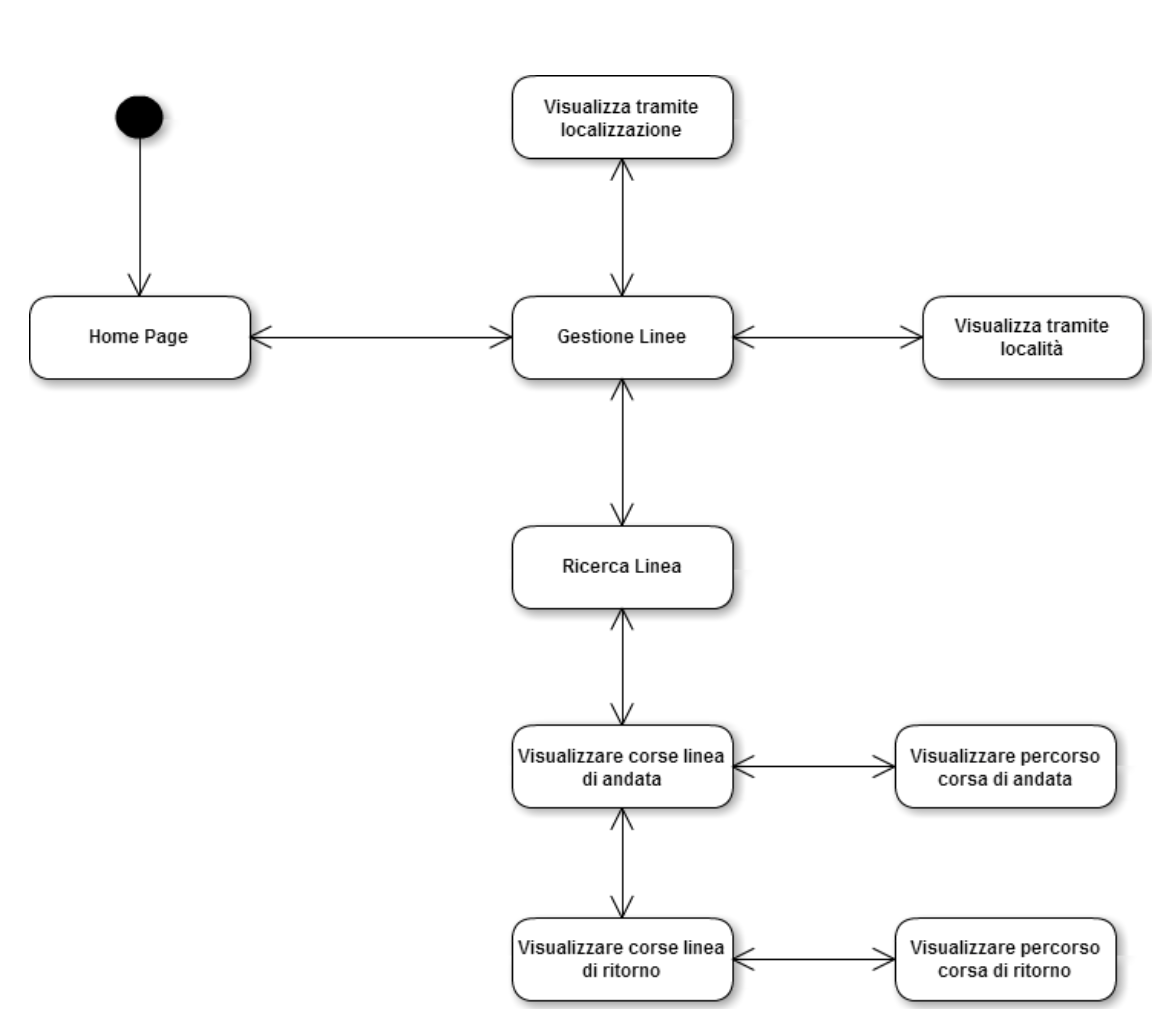
\includegraphics[scale=.4]{img/np.png}
\caption{Path navigazionale relativo alla gestione delle linee.}
\label{fig:np}
\end{figure} 

Come mostrato in Figura \ref{fig:np}, l'utente, a partire dalla Home Page dell'applicazione, pu\`{o} accedere alla funzionalit\`{a} di Gestione delle Linee, all\rq interno della quale \`{e} data la possibilit\`{a} di accedere i) alla visualizzazione delle linee tramite geo-localizzazione e  ii) visualizzazione della ricerca di una linea. Effettuando il caso d\rq uso mostrato in Figura \ref{fig:cd}, l\rq utente accede alla schermata di visualizzazione delle corse di andata per la linea selezionata, con la possibilit\`{a} di visualizzare anche la corsa di ritorno.\\

Infine, l'ultima parte dell\rq analisi dei requisiti \`{e} consistita nella definizione dei mockup delle funzionalit\`{a} identificate. In Figura \ref{fig:ui} \`{e} mostrato il mockup della funzionalit\`{a} di ricerca di una linea, implementato sulla base di una interfaccia per smartphone. 

\begin{figure}[h]
\centering
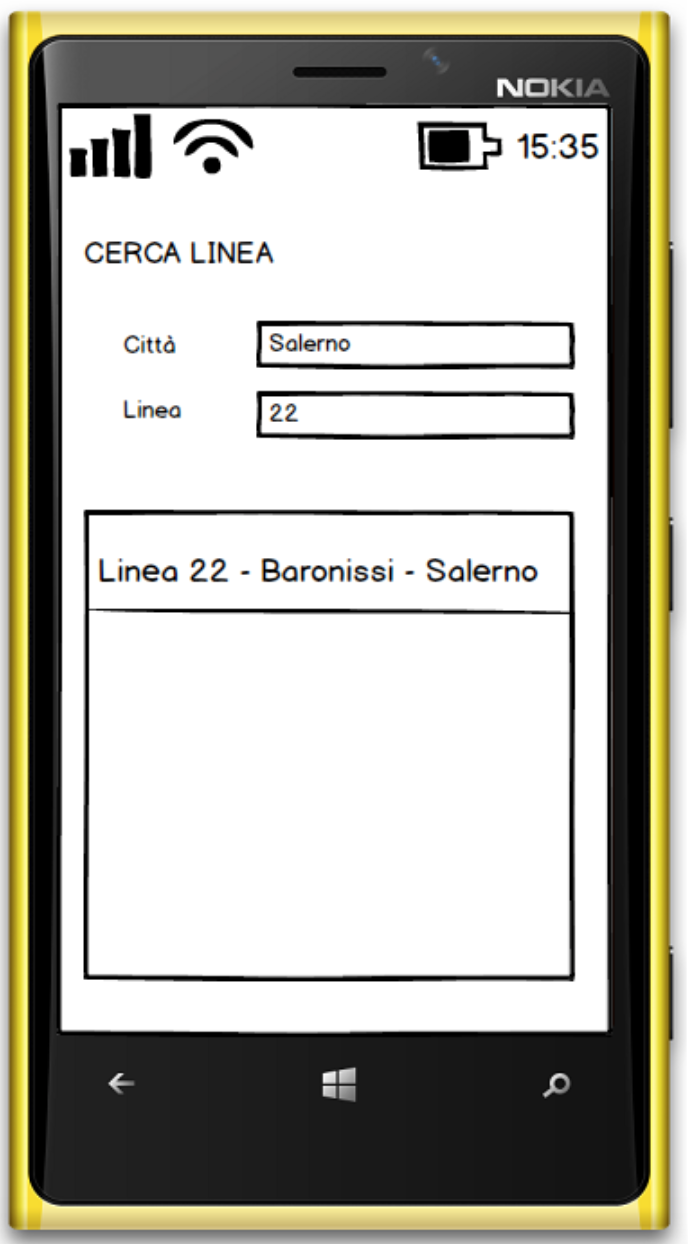
\includegraphics[scale=.3]{img/ui.png}
\caption{Screen Mockup della Funzionalit\`{a} di Ricerca di una Linea.}
\label{fig:ui}
\end{figure} 

La definizione degli screen mockup ci ha aiutato nella comprensione dei requisiti, ma anche nella definizione degli artefatti di basso livello descritti nelle successive sezioni. 

\subsection{Design}
Gli obiettivi principali della fase di design sono stati quelli di definire i) i design goal; ii) l\rq architettura dell\rq applicazione; e iii) il mapping hardware-software. Il primo step \`{e} consistito nella definizione degli obiettivi di design a partire dai requisiti non funzionali presenti nel documento di analisi e specifica dei requisiti. Sono stati identificate 4 categorie di design goal, di seguito riportati:\\

\noindent {\bf{DG-0 - Dependability criteria}}:  \emph{GoBus} garantir\`{a} il corretto svolgimento delle proprie funzioni, gestendo i vari errori logici (quelli derivanti da una negligenza da parte dell\rq utente), che potranno verificarsi durante l\rq utilizzo, ed eventuali attacchi alla sicurezza. Questo insieme di design goal comprende i requisiti di robustezza, affidabilit\`{a}, disponibilit\`{a} e sicurezza.\\
\noindent {\bf{DG-1 - Performance criteria}}:  Il sistema sar\`{a} usabile e leggero, in modo tale che, nel caso in cui più persone accedano al sistema contemporaneamente, questo non venga rallentato. In definitiva, il sistema dovr\`{a} garantire che le varie operazioni offerte vengano svolte entro un intervallo di tempo accettabile. Questo insieme di design goal comprende i tempi di risposta, il throughput, e i requisiti di memoria.\\
\noindent {\bf{DG-2 - Maintenance criteria}}:  \emph{GoBus} garantir\`{a} un alto grado di manutenibilit\`{a}. Questo insieme di design goal comprende l\rq estendibilit\`{a}, la modificabilit\`{a} e la tracciabilit\`{a} dei requisiti.\\
\noindent {\bf{DG-3 - End User criteria}}:  \emph{GoBus} garantir\`{a} la learnability e l\rq usabilit\`{a} del sistema.\\

Per quanto riguarda l\rq architettura del sistema, \emph{GoBus} sar\`{a} implementato in una architettura three-tier, e quindi tramite una suddivisione del sistema in tre livelli: i) \emph{presentation-layer}, \emph{application-layer} e \emph{storage-layer}. Il primo livello consiste di tutte le interfacce grafiche che consentiranno all\rq utente di poter dialogare con la logica di business, a sua volta implementata nell\rq application-layer. Infine, lo storage-layer contiene le componenti che consentono l\rq immagazzinamento dei dati.\\

Il successivo passo \`{e} consistito nella decomposizione del sistema in sottosistemi. In questo contesto, le metriche di coesione e accoppiamento rappresentano un importante strumento per poter definire una decomposizione che consenta a team di sviluppo separati di poter eseguire parallelamente diversi task. Nel nostro contesto, \`{e} stata definita la decomposizione mostrata in Figura \ref{fig:sd}.

\ref{fig:sd}
\begin{figure*}[tb]
\centering
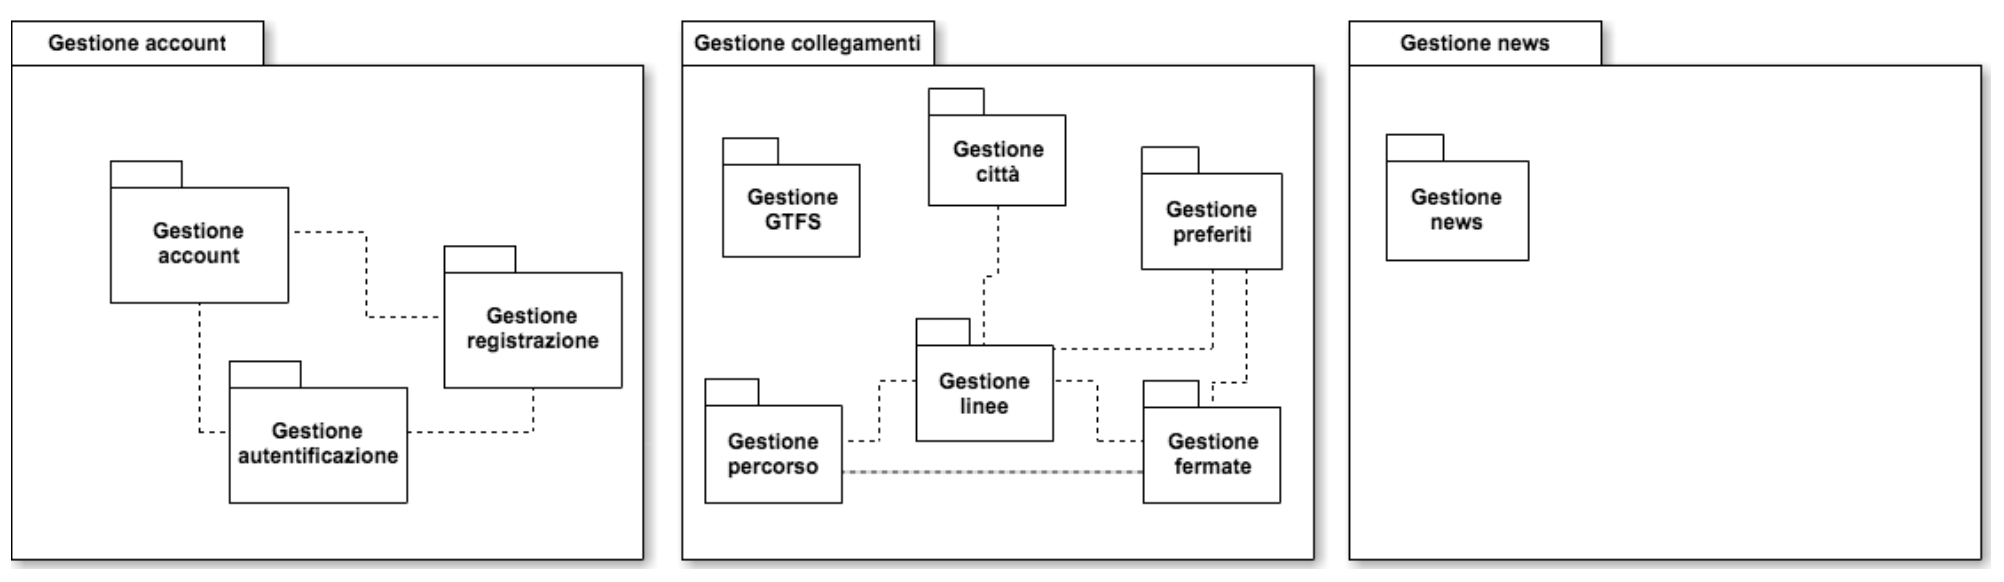
\includegraphics[scale=.4]{img/sd.png}
\caption{Decomposizione in Sottosistemi}
\label{fig:sd}
\end{figure*} 

Come \`{e} possibile vedere, \emph{GoBus} si compone di tre sottosistemi, che fanno riferimento i) alla gestione degli utenti (Gestione Account in Figura \ref{fig:sd}), ii) la gestione di tutti i dati relativi alle fermate, alle linee e ai percorsi (Gestione Collegamenti in Figura \ref{fig:sd}), e iii) la gestione dei preferiti, che rappresenta una componente a se stante nell\rq economia del sistema.\\

\begin{figure*}[tb]
\centering
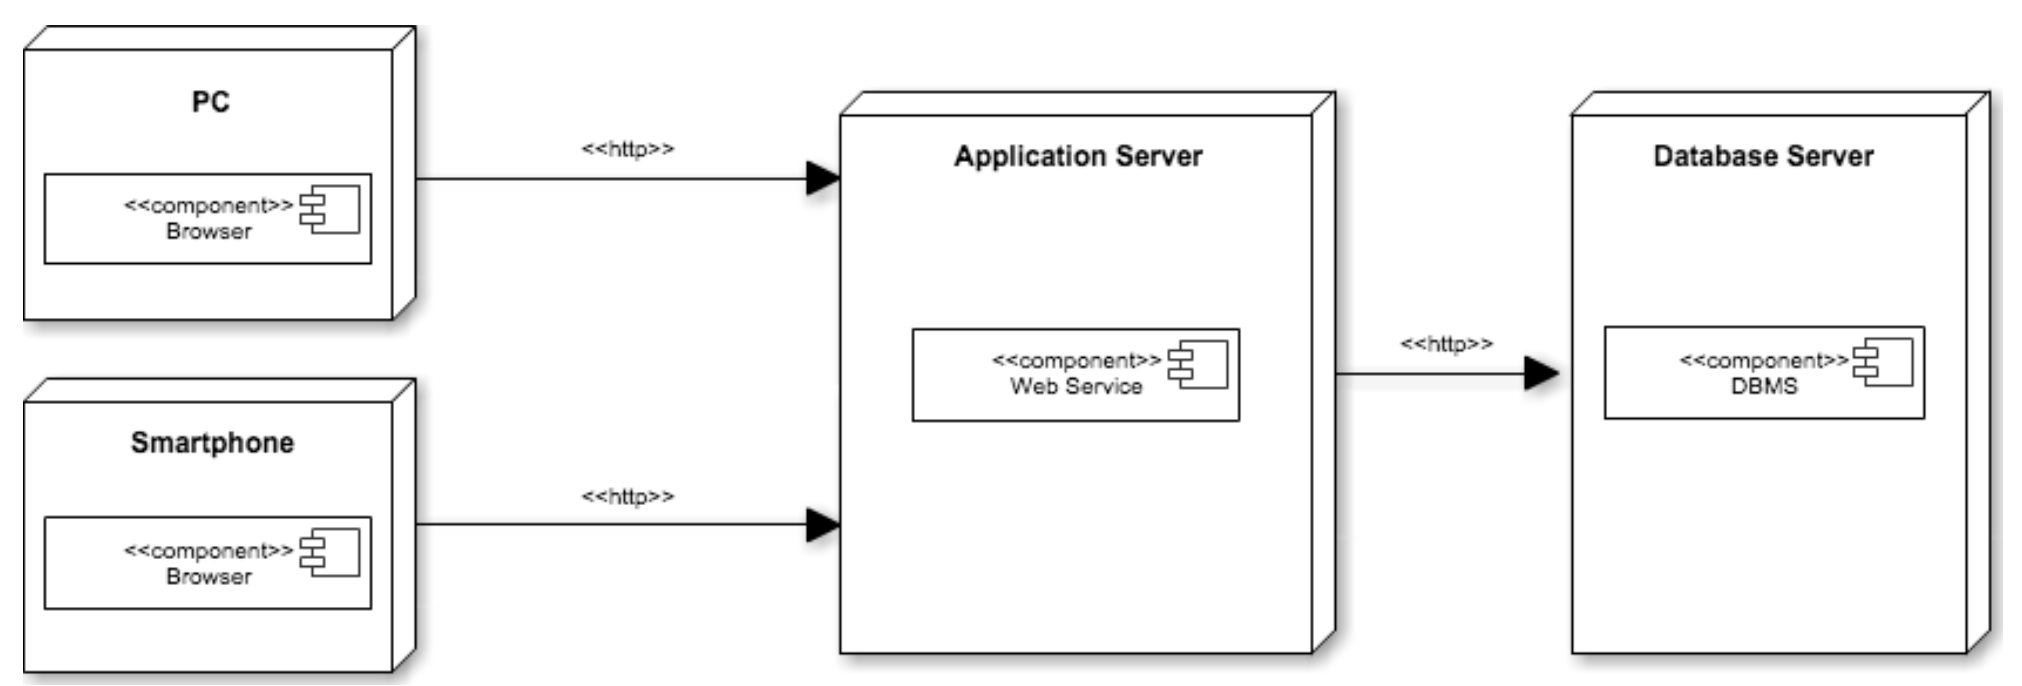
\includegraphics[scale=.4]{img/mhs.png}
\caption{Mapping Hardware/Software}
\label{fig:mhs}
\end{figure*} 

Infine, \`{e} stato definito il mapping hardware-software. Il Deployment Diagram fornisce un ausilio agli sviluppatori per quanto riguarda l\rq organizzazione delle componenti hardware e software del sistema \emph{GoBus}. In figura \ref{fig:mhs} possiamo vedere quali sono i nodi che interagiscono col sistema: Application Server e il Database Server. Le interfacce dei vari sottosistemi accedono ai pacchetti dell\rq Application Server, in cui risiedono gli oggetti di tipo control ed entity. L\rq accesso al database avviene tramite un sottosistema di storage, per garantire, anche, l\rq indipendenza di esso; infatti se sorgesse la necessit\`{a} di modificare una qualsiasi componente dell\rq interfaccia del sottosistema, non vi sarebbe il bisogno di apportare innumerevoli modifiche all\rq interno del sistema. La comunicazione tra i nodi avviene tramite protocollo HTTP.\\
Per quanto riguarda la base di dati del progetto \`{e} stata modellata sui file in formato General Transit Feed Specification Reference (GTFS). Questo formato \`{e} attualmente utilizzato dalle aziende di trasporto pubblico per la comunicazione dei dati, 
relativi ai servizi forniti, all\rq applicazione Google Transit. Questo consente alle aziende di 
fornire informazioni al progetto in modo facile e veloce, senza ridondanza di dati. 
Google fornisce le linee guida per la formattaione dei dati in questione, identificando un 
insieme di file. Tra questi ci sono file richiesti e file opzionali, ogni agenzia pu\`{o} decidere 
quali informazioni fornire in base alle proprie esigenze. \emph{GoBus} si propone di raggruppare 
in un\rq unica applicazione informazioni su tutte le agenzie di trasporto nazionali, per cui 
gestisce solo i dati obbligatori pi\`{u} alcune informazioni che non possono essere ignorate 
se fornite dall\rq agenzia, come ad esempio le eccezioni al calendario delle corse in giorni 
particolari. Questi file sono:\\

\begin{itemize}
\item {\bf{agency.txt}}: Uno o pi\`{u} agenzie di transito che forniscono i dati.\\
\item {\bf{stops.txt}}: Luoghi dove i bus fanno salire o scendere i passeggeri.\\
\item {\bf{routes.txt}}: Un percorso \`{e} un gruppo di viaggi che vengono visualizzati come un unico servizio.\\
\item {\bf{trips.txt}}: Viaggi per ogni itinerario. Un viaggio \`{e} una sequenza di due o pi\`{u} ferma relative ad un viaggio.\\
\item {\bf{stop\_ times.txt}}: Orario in cui un veicolo arriva ad una fermata, per ogni viaggio.\\
\item {\bf{calendar.txt}}: Date per i servizi che utilizzano un programma settimanale. Specifica quando viene avviato il servizio e finisce, oltre ai giorni della settimana in cui il servizio\`{e} disponibile.\\
\item {\bf{calendar\_ dates.txt}}: Date particolari in cui alcuni servizi subiscono una variazione.\\
\end{itemize}
All\rq interno degli stessi file, sono indicati dei campi obbligatori e dei campi opzionali.
Per comprendere la struttura della base di dati la \emph{figura 17} mostra il Diagramma Entit\`{a} Relazioni.



\begin{figure}[h]
\centering
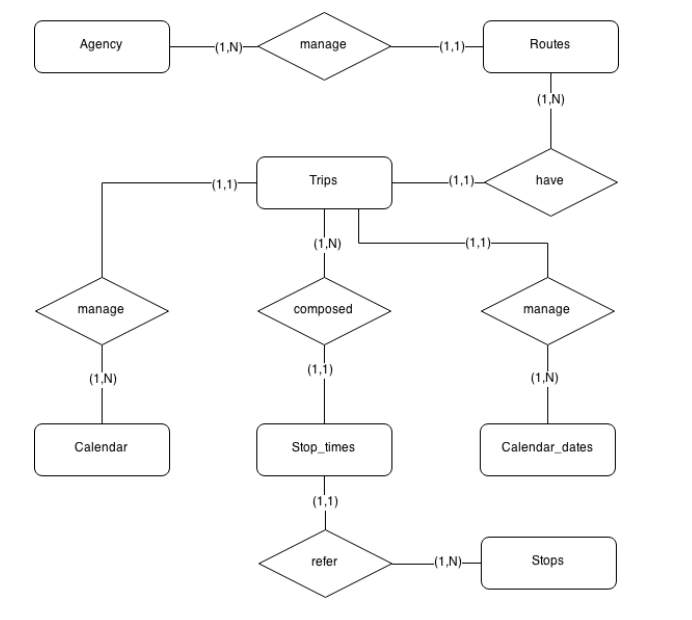
\includegraphics[scale=.4]{img/ER.png}
\caption{Diagramma Base di Dati}
\label{fig:ER}
\end{figure}

Infine, all\rq interno del design \`{e} stato analizzato il controllo degli accessi. 
Il dettaglio completo delle attivit\`{a} svolte in questa fase \`{e} nel documento di System Design allegato.

\subsection{Implementazione}
La fase di implementazione ha lo scopo di creare un prodotto software in grado di soddisfare tutti i requisiti individuati nela fase di pianificazione. Nell'ambito del progetto, tale attivit\`{a} viene svolta seguendo un modello evolutivo a prototipi. 

Il primo prototipo implementato ha lo scopo di comprendere al meglio i requisiti del web service e del portale web. In questa fase non \`{e} stato ritenuto necessario implementare il prototipo dell\rq applicazione mobile in quanto essa presenta gli stessi requisiti del portale web. 

In particolare il percorso di sviluppo \`{e} stato il seguente:\\
- Il web service \`{e} stato implementato in linguaggio php, con l\rq utilizzo di un framework esterno, Slim, il cui scopo \`{e} quello di mappare gli url inseriti dall\rq utente in query che presentino le informazioni dal database. In questo modo viene garantito che il web service utilizzi il protocollo rest. I risultati sono forniti in formato JSON.(\emph{figura 18}) \\
- La web application \`{e} stata realizzata utilizzando Bootstrap [Aggiungere referenza] e il framework jQuery [Aggiungere referenza]. Nel primo prototipo sono state implementate soltanto le funzionalit\`{a} principali, tralasciando la gestione dell\rq utente e degli avvisi.(\emph{figura 19}) \\

\begin{figure*}[tb]
\centering
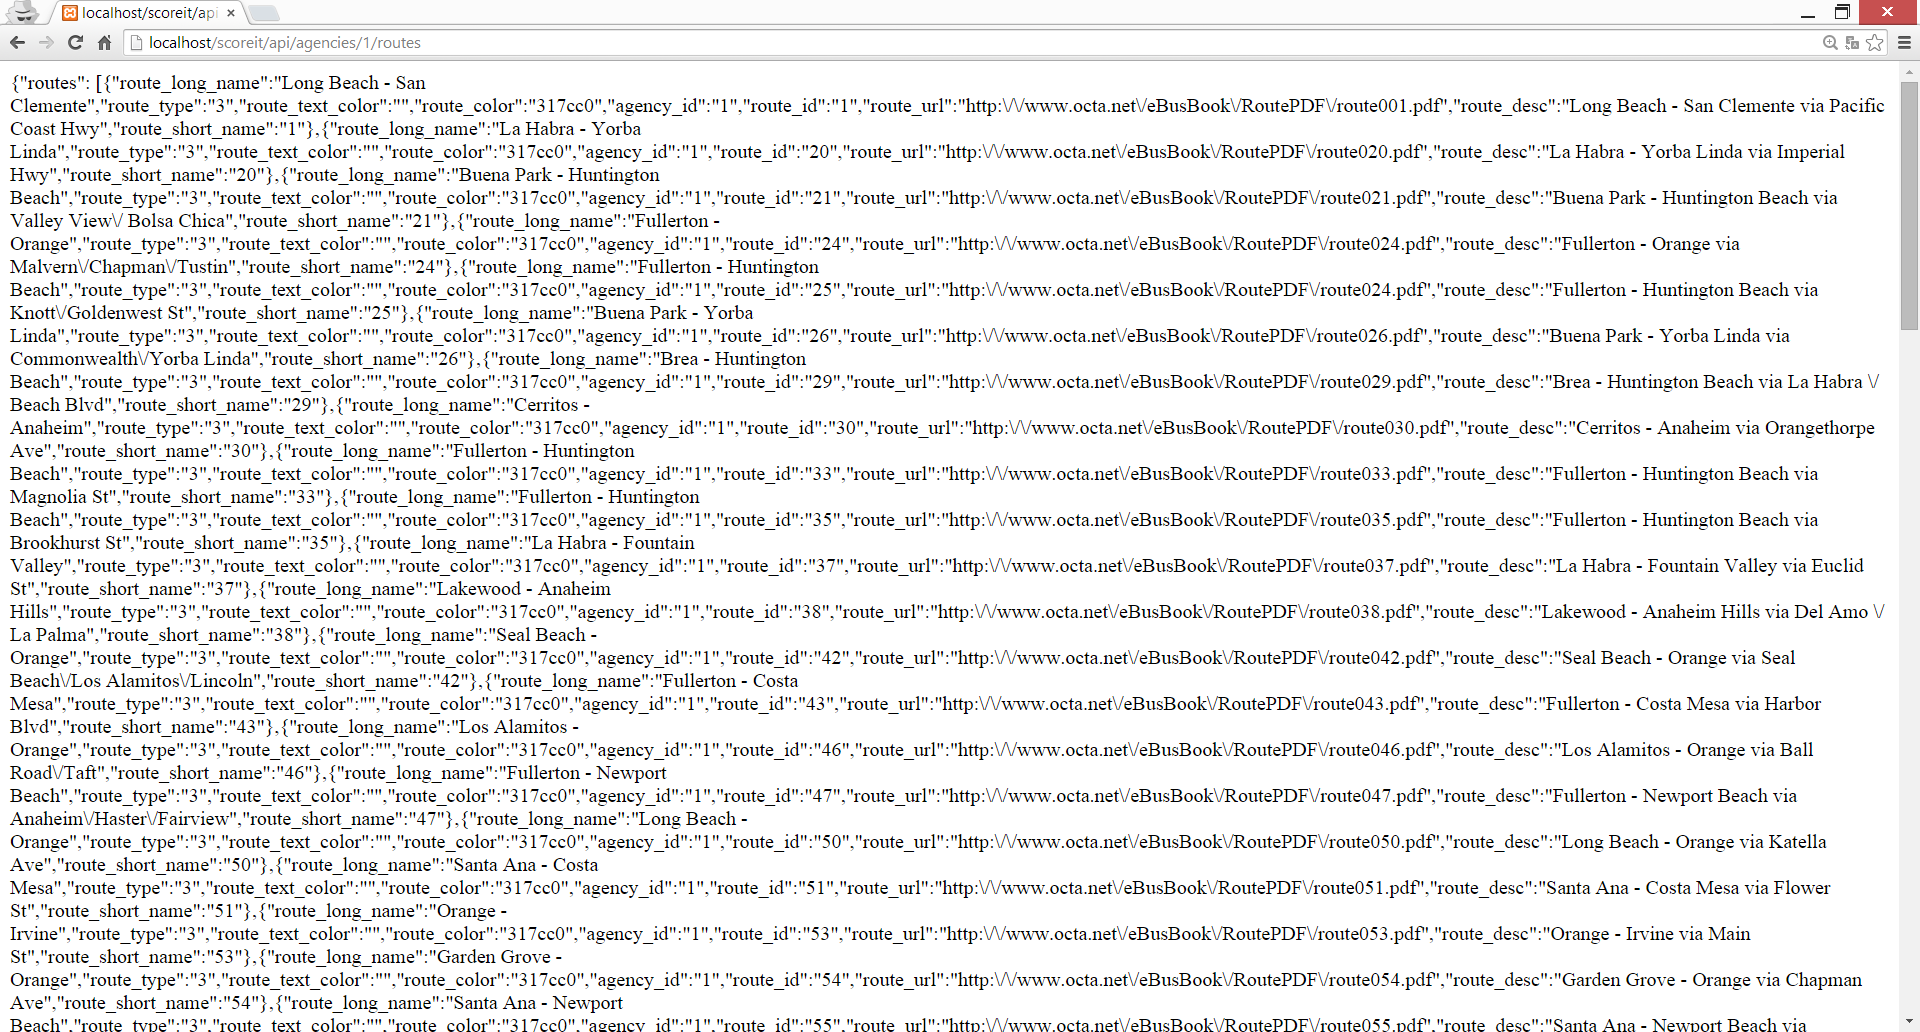
\includegraphics[scale=.3]{img/19.png}
\caption{Esempio risultato ricerca linea su Web service }
\label{fig:mhs}
\end{figure*} 

\begin{figure*}[tb]
\centering
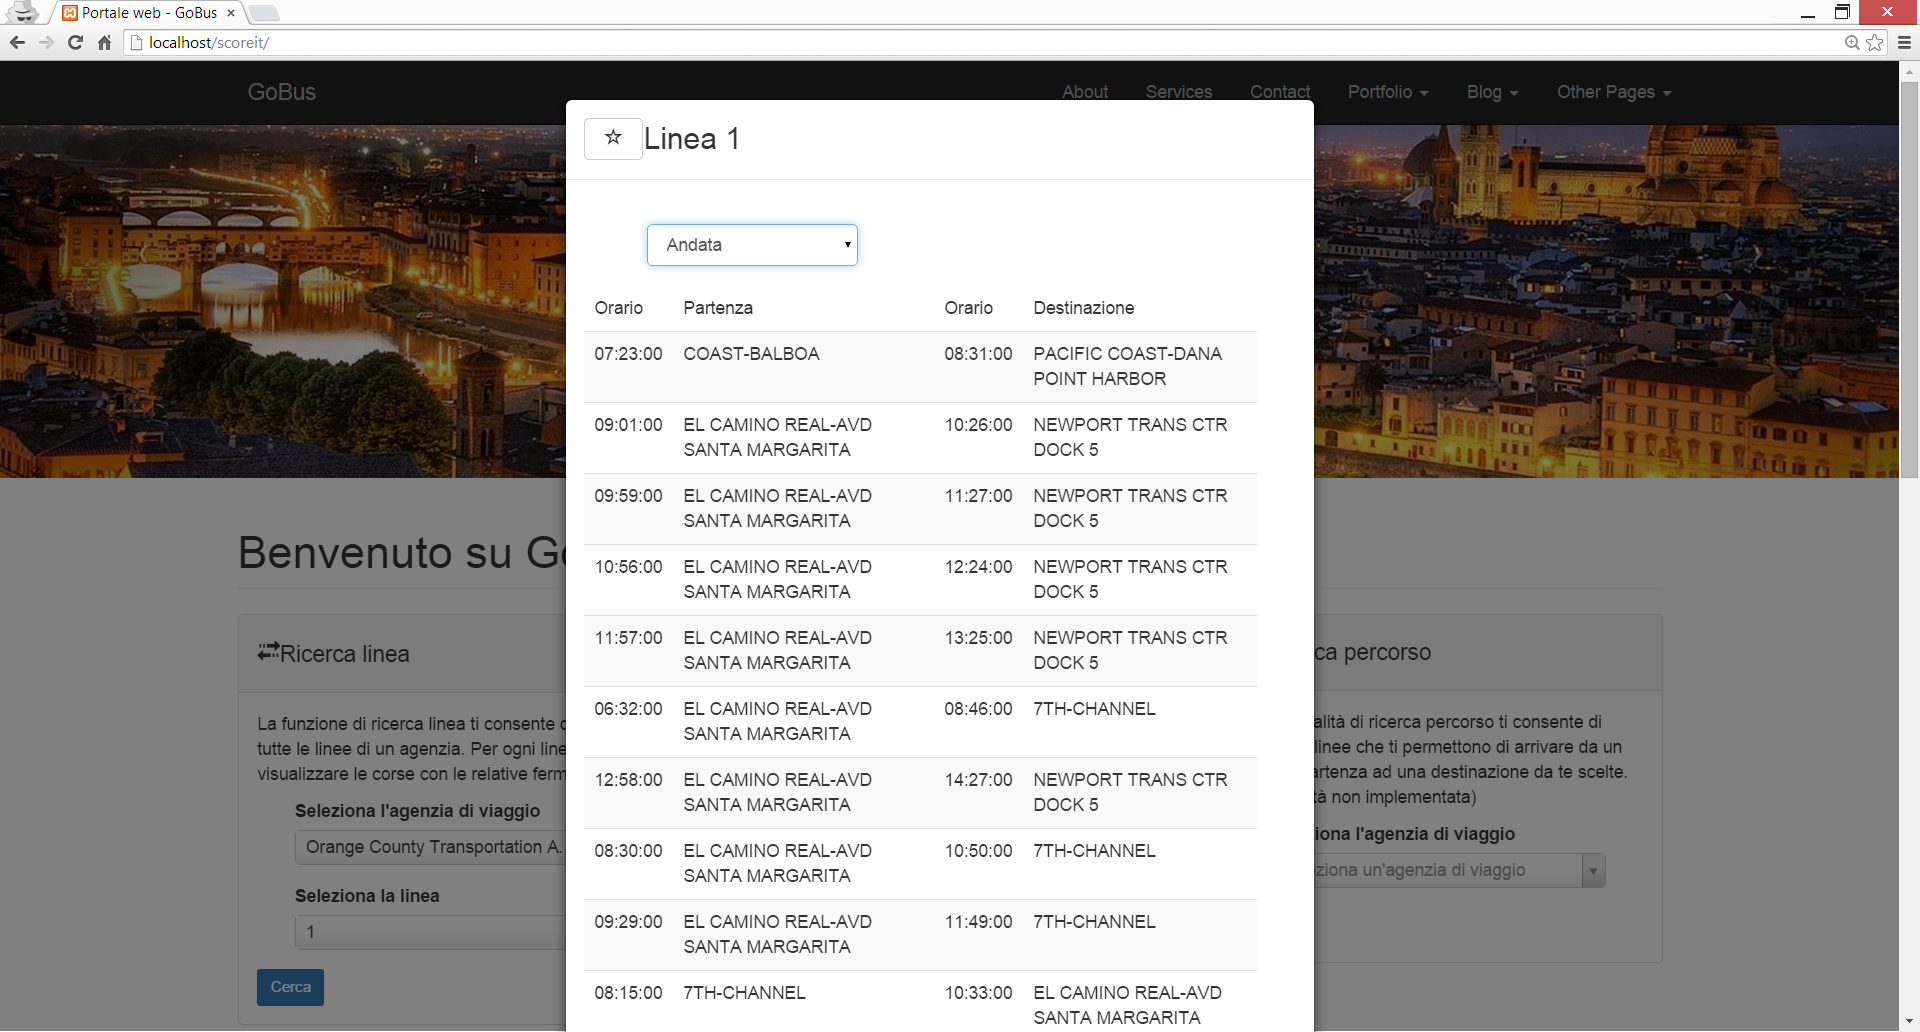
\includegraphics[scale=.3]{img/20.png}
\caption{Esempio risultato ricerca linea su Web application }
\label{fig:mhs}
\end{figure*} 


Analisi:\\
Il primo prototipo ha evidenziato di essere inefficiente in quanto alcune query rilevanti hanno mostrato tempi di risposta troppo elevati. A tal proposito sono state valutate diverse alternative, tra cui una diversa architettura della base di dati e l\rq utilizzo di un database ad oggetti come MongoDB\footnote{http://www.mongodb.org/ }.\\
Il portale web ha chiarito il modo di visualizzazione delle informazioni per quanto riguarda la gestione delle fermate e la gestione delle linee. 



\subsection{Testing}
La pianificazione del testing prevede tre tipologie di test: testing di unit\`{a}, testing di integrazione e testing di sistema.\\
In merito al testing di unit\`{a}, il processo di testing per il progetto "GoBus" verr\`{a} sottoposto ad una tipologia di testing di tipo black-box, ovvero, si stresser\`{a} il sistema dal punto di vista funzionale, analizzando e confrontando gli output derivanti dagli input immessi, con gli output attesi. In combinazione con il testing black-box sar\`{a} utilizzato category partition. Questa tecnica permette di dividere i possibili input in gruppi, i cui elementi generano output logicamente simili. Tali gruppi, identificati come classi di equivalenza, saranno identificati e utilizzati in modo da eseguire almeno un test per ognuno di essi. Per agevolare il testing di regressione, in seguito alla modifica delle componenti software verr\`{a} utilizzato un framework adatto.\\
Relativamente al testing di integrazione, verr\`{a} adottata una strategia di tipo bottom-up. In sintesi si testeranno le componenti del sistema partendo dal layer pi\`{u} in basso nella gerarchia. L\rq implementazione di tale strategia prevede la costruire di driver test, ovvero di classi che utilizzino in maniera banale le componenti sotto test.\\
Il testing di sistema verr\`{a} effettuato mediante l\rq analisi empirica statica, ovvero confrontando il comportamento del sistema in esecuzione in relazione al comportamento atteso.\\

\begin{figure}[h]
\centering
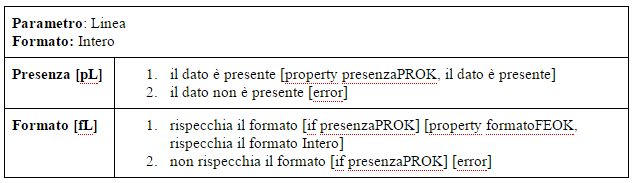
\includegraphics[scale=.6]{img/21.png}
\caption{Esempio Test case }
\label{fig:mhs}
\end{figure}  

\begin{figure}[h]
\centering
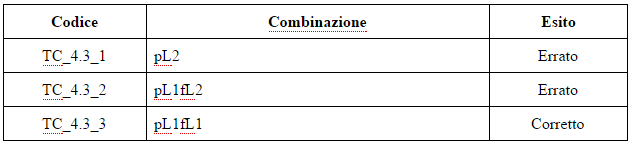
\includegraphics[scale=.6]{img/22.png}
\caption{Esempio combinazione Test}
\label{fig:mhs}
\end{figure} 

\begin{figure}[h]
\centering
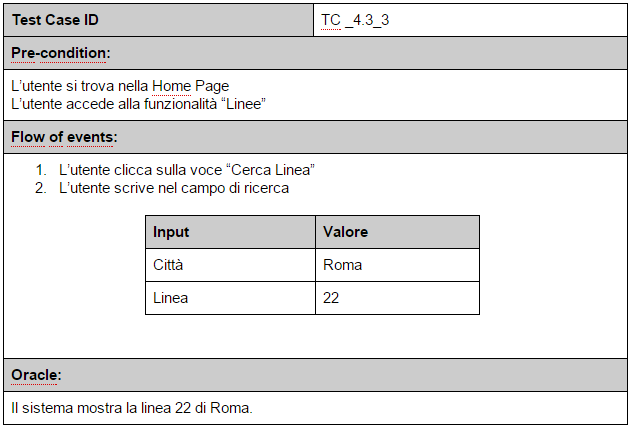
\includegraphics[scale=.6]{img/23.png}
\caption{Esempio category partition }
\label{fig:mhs}
\end{figure} 

\subsection{Rilascio}
Il prototipo viene rilasciato. Si pu\`{o} fare riferimento al video che mostra la demo dell\rq applicazione, (in allegato nel materiale consegnato) e al file zip contenente il codice dell\rq implementazione.



\section{Conclusioni e Sviluppi Futuri}
In conclusione, ripercorriamo tutti i passi del ciclo di vita del progetto, che ha previsto non solo un ciclo di vita ingegneristico, ma anche anche manageriale. Il primo passo \`{e} stato quello di adottare i 5 gruppi di processi descritti nel PMBOK: \emph{initiating, planning, executing, monitoring and controlling, closing}.\\
Il documento di Statement of Work \`{e} stato il punto di partenza del progetto. Nel documento, stilato insieme agli stakeholder, sono stati inclusi i \emph{Business Needs}, ovvero le esigenze di business. Ad ognuna di queste \`{e} stato associato un piano di risoluzione.
Si \`{e} quindi proceduto con la fase di pianificazione, definendo il documento principale, ovvero il \emph{Software Project Management Plan} (SPMP). Questo documento include tutte le informazioni provenienti dalle dieci aree di conoscenza del project manangement. Particolarmente rilevanti, sono stati il \emph{Requirements Management Plan}, per la gestione dei requisiti, il \emph{Software Configuration Management Plan} per l\rq implementazione del Configuration Management, il \emph{Quality Plan} e il \emph{Risk Management Plan}.\\
Molti documenti sono stati scritti in contemporanea e alcuni hanno subito diverse revisioni (ad esempio il SPMP).
A partire dal \emph{Requirements Management Plan} \`{e} stato quindi possibile effettuare la raccolta requisiti e l\rq analisi degli stessi. Ovviamente molti di questi requisiti sono stati sviluppati a partire dalle business needs iniziali. 
Nella fase di planning si \`{e} sono state quindi pianificate le fasi di esecuzione, monitoraggio e controllo.\\
Durante la fase di esecuzione sono stati prodotti documenti fondamentali per quanto concerne il processo d\rq Ingegneria del Software quali il System Design Document (SDD) e l\rq Object Design Document (ODD) sviluppati partendo dal documento di analisi dei requisiti.
Allo stato attuale, la fase di implementazione \`{e} stata considerata un\rq attivit\`{a} secondaria rispetto alla produzione di documentazione, in quanto ci si \`{e} limitati alla sola creazione di un prototipo di web service e di application web, allegato alla documentazione.
Nella fase di chiusura, che avverr\`{a} a fine progetto, ci sar\`{a} la release dei prodotti con conseguente post-mortem review in cui saranno specificate le best practices adottate e le lessons learned.\\
I prossimi passi da fare riguarderanno:
\begin{itemize}
\item l\rq implementazione dell\rq applicazione mobile per la piattaforma Windows Phone;
\item l\rq applicazione web,a supporto delle agenzie di trasporti;
\item l\rq implementazione completa del web service attraverso un protocollo di comunicazione restful. Il servizio sar\`{a} implementato usando tecnologie pi\`{u} performanti, quali ad esempio un DBMS ad oggetti.
\end{itemize}
\begin{thebibliography}{1}

\bibitem{PMBOK}
Project Management Institute. (2004). A guide to the project management body of knowledge (PMBOK guide). Newtown Square, Pa, Project Management Institute.

\bibitem{ITIL}
It Service Management: A Guide for Itil Foundation Exam Candidates (Second Edition) di Ernest Brewster, Richard Griffiths, Aidan Lawes, John Sansbury.


\end{thebibliography}




% that's all folks
\end{document}


